\documentclass[10pt,twocolumn]{article}
\usepackage{simpleConference}
\usepackage[T1]{fontenc}
\usepackage{times,graphicx,lineno}
\setlength{\textheight}{6.7in}
\setlength{\parskip}{5pt}
\pagestyle{plain}
\hyphenpenalty=10000
\exhyphenpenalty=10000
\begin{document}
\title{Controlled academic layout study}
\author{Alex Researcher}
\date{}
\maketitle
\linenumbers
\section{Introduction}
The experiment studies how page layout changes the recovery of scientific prose from a document. Each page keeps the same research content while the positions of surrounding objects change.


A reliable reader follows the left column before moving to the beginning of the right column. The reading sequence must preserve the relationship between an observation and its explanation.


\begin{table}[t]
\centering
\begin{tabular*}{0.46\textwidth}{@{\extracolsep{\fill}}lr}
\hline
Treatment & Response \\
\hline
Control & 12.4 \\
Revised & 18.7 \\
Repeated & 17.9 \\
\hline
\end{tabular*}
\caption{Treatment measurements from the controlled study.}
\end{table}

The sampling method selects independent measurements from several sites with different local conditions. We retain the original measurements so that later comparisons use the same evidence throughout the study.


The control group receives the standard treatment while the experimental group receives the revised treatment. The difference between these groups estimates the effect of the intervention under matched conditions.


The measured temperature remains near 25 degrees during each trial despite small changes in room pressure. These numeric observations belong to ordinary prose and must not disappear with the printed line numbers.


\begin{figure}[t]
\centering
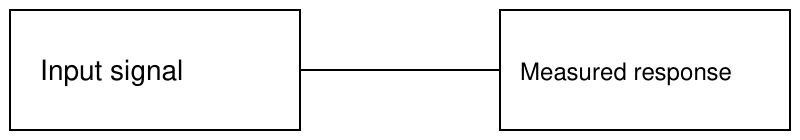
\includegraphics[width=0.46\textwidth,height=55pt]{pathway.png}
\caption{Measurement pathway used during the controlled study.}
\end{figure}

The calibration procedure compares each sensor with a stable reference instrument before data collection begins. This procedure reduces systematic error without changing the order of the measurements in the final report.


\section{Results}
The primary outcome improves across the sampled sites and remains consistent during repeated observations. The secondary outcome varies between sites because the local environment changes the available resources.


A narrow table presents a small set of measurements without becoming part of the surrounding paragraph. A wide illustration separates regions of prose but does not change the order of the sentences within them.


The analysis retains unusual findings because a rare observation can reveal a limitation of the proposed method. The interpretation distinguishes this limitation from random variation in the measurements collected during the study.


The final comparison supports the proposed method for the measured conditions but not for every possible setting. Further experiments must examine other conditions before the same conclusion applies to a broader population.


The discussion ends with a complete statement before the bibliography begins on the following page. Bibliographic entries identify earlier publications and do not belong to the prose selected for highlighting.


\clearpage
\nolinenumbers
\section*{References}
[1] Smith, J. 2021. Reliable measurements in experimental research. Journal of Controlled Studies, volume 12, pages 45 to 67.

[2] Jones, A. 2022. Reading order in scientific documents. Proceedings of the Document Analysis Conference, pages 120 to 135.

[3] Brown, C. 2023. Calibration methods for independent sensors. Journal of Measurement Science, volume 8, pages 201 to 219.
\end{document}
